\documentclass[aspectratio=169,14pt]{beamer}

\usepackage{hyperref}
\usepackage{biblatex}

\usepackage{amsmath}
\usepackage{bm}

\addbibresource{references.bib}

\usepackage{varwidth}
\usepackage{tikz}
\usetikzlibrary{tikzmark}

\usepackage{amsmath,amsthm,amssymb}
\usepackage{cleveref}
\usepackage{comment}

% Allowing page breaks in align
\allowdisplaybreaks

% Other commands
\newcommand{\loss}[1]{\ell\ifthenelse{\isempty{#1}{}}{}{\!\left(#1\right)}}
\newcommand{\negspace}[1]{\phantom{\hspace*{-#1}}}

% Math operators
\DeclareMathOperator*{\argmin}{arg\,min}
\DeclareMathOperator*{\argmax}{arg\,max}
\DeclareMathOperator*{\expect}{\mathbb{E}}
\DeclareMathOperator*{\prob}{\mathbb{P}}

% Vectors
\newcommand{\mydefv}[1]{\expandafter\newcommand\csname v#1\endcsname{\mathbf{#1}}}
\newcommand{\mydefallv}[1]{\ifx#1\mydefallv\else\mydefv{#1}\expandafter\mydefallv\fi}
\mydefallv abcekmosuvwxyz\mydefallv

% Vectors symbols
\newcommand{\mydefvsym}[1]{\expandafter\newcommand\csname v#1\endcsname{\boldsymbol{\csname #1\endcsname}}}
\newcommand{\mydefallvsym}[1]{\ifx#1\mydefallvsym\else\mydefvsym{#1}\expandafter\mydefallvsym\fi}
\mydefallvsym {sigma}{alpha}{gamma}{mu}{rho}\mydefallvsym

% Set
\newcommand{\mydefset}[1]{\expandafter\newcommand\csname set#1\endcsname{{#1}}}
\newcommand{\mydefallset}[1]{\ifx#1\mydefallset\else\mydefset{#1}\expandafter\mydefallset\fi}
\mydefallset BFHPSTVYZ\mydefallset

% Distribution over a space
\newcommand{\mydefdistr}[1]{\expandafter\newcommand\csname distr#1\endcsname{\mathcal{D}_{\csname space#1\endcsname}}}
\newcommand{\mydefalldistr}[1]{\ifx#1\mydefalldistr\else\mydefdistr{#1}\expandafter\mydefalldistr\fi}
\mydefalldistr DHNSTVXZ\mydefalldistr

% Empirical Distribution
\newcommand{\mydefedistr}[1]{\expandafter\newcommand\csname edistr#1\endcsname{\widehat{\mathcal{D}}_{\csname space#1\endcsname}}}
\newcommand{\mydefalledistr}[1]{\ifx#1\mydefalledistr\else\mydefedistr{#1}\expandafter\mydefalledistr\fi}
\mydefalledistr WZ\mydefalledistr

% Space
\newcommand{\mydefspace}[1]{\expandafter\newcommand\csname space#1\endcsname{\mathcal{#1}}}
\newcommand{\mydefallspace}[1]{\ifx#1\mydefallspace\else\mydefspace{#1}\expandafter\mydefallspace\fi}
\mydefallspace DFGHKLMNPSRTUVXYZ\mydefallspace

% Function
\newcommand{\mydeff}[1]{\expandafter\newcommand\csname f#1\endcsname[2][]{#1##1\ifthenelse{\equal{##2}{}}{}{\!\left(##2\right)}}}
\newcommand{\mydefallf}[1]{\ifx#1\mydefallf\else\mydeff{#1}\expandafter\mydefallf\fi}
\mydefallf cdfqghklsuyzCFGHKLMRT\mydefallf

% Function symbols
\newcommand{\mydeffsym}[1]{\expandafter\newcommand\csname f#1\endcsname[2][]{\csname #1\endcsname##1\ifthenelse{\equal{##2}{}}{}{\!\left(##2\right)}}}
\newcommand{\mydefallfsym}[1]{\ifx#1\mydefallfsym\else\mydeffsym{#1}\expandafter\mydefallfsym\fi}
\mydefallfsym {Omega}{phi}{epsilon}{delta}{eta}{theta}{nu}{tildeh}{kappa}{rho}\mydefallfsym

% Number Set
\newcommand{\mydefnset}[1]{\expandafter\newcommand\csname nset#1\endcsname{\mathbb{#1}}}
\newcommand{\mydefallnset}[1]{\ifx#1\mydefallnset\else\mydefnset{#1}\expandafter\mydefallnset\fi}
\mydefallnset CNRSZ\mydefallnset

% Norm
\newcommand{\normTwo}[1]{\left\|#1\right\|_2}
\newcommand{\normF}[1]{\left\|#1\right\|_\mathcal{F}}
\newcommand{\normOne}[1]{\left\|#1\right\|_1}
\newcommand{\normNuc}[1]{\left\|#1\right\|_\mathcal{*}}
\newcommand{\normMax}[1]{\left\|#1\right\|_\infty}
\newcommand{\norm}[1]{\left\|#1\right\|}
\newcommand{\abs}[1]{\left|#1\right|}
\newcommand{\hinge}[1]{\left[#1\right]_+}
\newcommand{\dotprod}[2]{\left\langle#1,#2\right\rangle}
\newcommand{\trace}[1]{\text{Tr}\left(#1\right)}
\newcommand{\inv}[1]{\left( #1 \right)^{-1}}
\newcommand{\bigO}[1]{\mathcal{O}\left( #1 \right)}

\newcommand{\scalar}[2]{\langle #1, #2 \rangle}

% Indic
\newcommand{\indic}[1]{\mathbb{I}_{ #1}}

% Ceil and Floor
\newcommand{\ceil}[1]{{\left\lceil #1 \right\rceil}}
\newcommand{\floor}[1]{{\left\lfloor #1 \right\rfloor}}

% Environments
\newtheorem{myth}{Theorem}
\newtheorem*{myth*}{Theorem}
\newtheorem{mycor}{Corollary}
\newtheorem*{mycor*}{Corollary}
\newtheorem{mylem}{Lemma}
\newtheorem*{mylem*}{Lemma}
\newtheorem{mydef}{Definition}
\newtheorem{myex}{Example}
\newtheorem*{myex*}{Example}
\newtheorem{myprop}{Proposition}

\newtheorem{myrmq}{Remark}
\newtheorem*{myrmq*}{Remark}


% Bold font in theorem headings
\makeatletter
\def\th@plain{%
  \thm@notefont{}% same as heading font
  \itshape % body font
}
\def\th@definition{%
  \thm@notefont{}% same as heading font
  \normalfont % body font
}
\makeatother
\newcommand{\targetlabel}[1][]{\fy{#1}}
\newcommand{\fairlabel}[1][]{\fs{#1}}
\newcommand{\DDP}[1][]{\text{DDP}\!\left(#1\right)}
\newcommand{\DEO}[1][]{\text{DEO}\!\left(#1\right)}
\newcommand{\eDDP}[1][]{\widehat{\text{DDP}}\!\left(#1\right)}
\newcommand{\eDEO}[1][]{\widehat{\text{DEO}}\!\left(#1\right)}
\newcommand{\eDDPm}[1][]{\widehat{\text{DDP}}^+}
\newcommand{\eDDPp}[1][]{\widehat{\text{DDP}}^-}
\newcommand{\lrDDP}[1][]{\text{LR}_{{\text{DDP}}}\!\left(#1\right)}
\newcommand{\srDDP}[1][]{\text{SR}_{{\text{DDP}}}\!\left(#1\right)}
\newcommand{\lrDEO}[1][]{\text{LR}_{{\text{DEO}}}\!\left(#1\right)}
\newcommand{\lreDDP}[1][]{\text{LR}_{\widehat{\text{DDP}}}\!\left(#1\right)}
\newcommand{\sreDDP}[1][]{\text{SR}_{\widehat{\text{DDP}}}\!\left(#1\right)}
\newcommand{\lreDEO}[1][]{\text{LR}_{\widehat{\text{DEO}}}\!\left(#1\right)}
\newcommand{\CCreDDP}[1][]{\text{CCR}_{\widehat{\text{DDP}}}\!\left(#1\right)}
\newcommand{\crDDP}[1][]{\text{R}_{\text{DDP}}\!\left(#1\right)}
\newcommand{\creDDP}[1][]{\text{R}_{\widehat{\text{DDP}}}\!\left(#1\right)}
\newcommand{\CCreDEO}[1][]{\text{CCR}_{\widehat{\text{DEO}}}\!\left(#1\right)}
\newcommand{\DDPkappa}[1][]{\text{DDP}_{\kappa}\!\left(#1\right)}
\newcommand{\DDPdelta}[1][]{\text{DDP}_{\delta}\!\left(#1\right)}
\newcommand{\eDDPkappa}[1][]{\widehat{\text{DDP}}_{\kappa}\!\left(#1\right)}
\newcommand{\eDDPdelta}[1][]{\widehat{\text{DDP}}_{\delta}\!\left(#1\right)}
\newcommand{\eDDPkappam}[1][]{\widehat{\text{DDP}}_{\kappa}^-}
\newcommand{\eDDPdeltap}[1][]{\widehat{\text{DDP}}_{\delta}^+}
\newcommand{\targeteps}{\varepsilon}
\newcommand{\faireps}{\varepsilon_f}
\newcommand{\targetmargin}{\gamma}
\newcommand{\fairnessSlack}{\mu}
\newcommand{\reasonable}{\tau}
\newcommand{\highmarginFraction}{\nu}
\newcommand{\learningProblem}{\mathrm{P}}
\newcommand{\map}[2]{\phi^{#1}\!\left(#2\right)}
\newcommand{\sign}[1]{\text{sign}\!\left(#1\right)}
\newcommand{\trueR}[1]{L\!\left(#1\right)}
\newcommand{\empR}[1]{\widehat{L}\!\left(#1\right)}
\newcommand{\reg}[1]{\fOmega{#1}}
\newcommand{\normal}[1]{\mathcal{N}\!\left(#1\right)}
\newcommand{\rad}[2]{\mathfrak{R}_{#1}\!\left(#2\right)}

\newcommand{\fairscalar}[1][]{\fq{#1}}
\newcommand{\phimax}{\phi_{\mathrm{max}}}

\newcommand{\cause}[1]{&{\color{gray}\downarrow{}\;{\small \text{#1}}} \nonumber\\}

\newcommand{\priv}{\mathrm{priv}}
\newcommand{\refer}{\mathrm{ref}}


% accuracy
\DeclareMathOperator*{\Acc}{Acc}

%%% Local Variables:
%%% mode: latex
%%% TeX-master: "main"
%%% End:

%%%%%%%%%%%%%%%%%%%%%%%%%%%%%%%%%%%%%%%%%%%%%%%%%%%%%%%%%%%%%%%%%%%%%%%%%%%%%%%
% Style mathbb
%%%%%%%%%%%%%%%%%%%%%%%%%%%%%%%%%%%%%%%%%%%%%%%%%%%%%%%%%%%%%%%%%%%%%%%%%%%%%%%

% cal letters
\newcommand{\cA}{\mathcal{A}}
\newcommand{\cB}{\mathcal{B}}
\newcommand{\cC}{\mathcal{C}}
\newcommand{\cD}{\mathcal{D}}
\newcommand{\cE}{\mathcal{E}}
\newcommand{\cF}{\mathcal{F}}
\newcommand{\cG}{\mathcal{G}}
\newcommand{\cH}{\mathcal{H}}
\newcommand{\cI}{\mathcal{I}}
\newcommand{\cJ}{\mathcal{J}}
\newcommand{\cK}{\mathcal{K}}
\newcommand{\cL}{\mathcal{L}}
\newcommand{\cM}{\mathcal{M}}
\newcommand{\cN}{\mathcal{N}}
\newcommand{\cO}{\mathcal{O}}
\newcommand{\cP}{\mathcal{P}}
\newcommand{\cQ}{\mathcal{Q}}
\newcommand{\cR}{\mathcal{R}}
\newcommand{\cS}{\mathcal{S}}
\newcommand{\cT}{\mathcal{T}}
\newcommand{\cU}{\mathcal{U}}
\newcommand{\cV}{\mathcal{V}}
\newcommand{\cW}{\mathcal{W}}
\newcommand{\cX}{\mathcal{X}}
\newcommand{\cY}{\mathcal{Y}}
\newcommand{\cZ}{\mathcal{Z}}

% bold letters (upper case)
\newcommand{\bfA}{\mathbf{A}}
\newcommand{\bfB}{\mathbf{B}}
\newcommand{\bfC}{\mathbf{C}}
\newcommand{\bfD}{\mathbf{D}}
\newcommand{\bfE}{\mathbf{E}}
\newcommand{\bfF}{\mathbf{F}}
\newcommand{\bfG}{\mathbf{G}}
\newcommand{\bfH}{\mathbf{H}}
\newcommand{\bfI}{\mathbf{I}}
\newcommand{\bfJ}{\mathbf{J}}
\newcommand{\bfK}{\mathbf{K}}
\newcommand{\bfL}{\mathbf{L}}
\newcommand{\bfM}{\mathbf{M}}
\newcommand{\bfN}{\mathbf{N}}
\newcommand{\bfO}{\mathbf{O}}
\newcommand{\bfP}{\mathbf{P}}
\newcommand{\bfQ}{\mathbf{Q}}
\newcommand{\bfR}{\mathbf{R}}
\newcommand{\bfS}{\mathbf{S}}
\newcommand{\bfT}{\mathbf{T}}
\newcommand{\bfU}{\mathbf{U}}
\newcommand{\bfV}{\mathbf{V}}
\newcommand{\bfW}{\mathbf{W}}
\newcommand{\bfX}{\mathbf{X}}
\newcommand{\bfY}{\mathbf{Y}}
\newcommand{\bfZ}{\mathbf{Z}}

% bold letters (lower case)
\newcommand{\bfa}{\mathbf{a}}
\newcommand{\bfb}{\mathbf{b}}
\newcommand{\bfc}{\mathbf{c}}
\newcommand{\bfd}{\mathbf{d}}
\newcommand{\bfe}{\mathbf{e}}
\newcommand{\bfbf}{\mathbf{f}}
\newcommand{\bfg}{\mathbf{g}}
\newcommand{\bfh}{\mathbf{h}}
\newcommand{\bfi}{\mathbf{i}}
\newcommand{\bfj}{\mathbf{j}}
\newcommand{\bfk}{\mathbf{k}}
\newcommand{\bfl}{\mathbf{l}}
%\newcommand{\fbm}{\mathbf{m}} % not compatible with bm package.
\newcommand{\bfn}{\mathbf{n}}
\newcommand{\bfo}{\mathbf{o}}
\newcommand{\bfp}{\mathbf{p}}
\newcommand{\bfq}{\mathbf{q}}
\newcommand{\bfr}{\mathbf{r}}
\newcommand{\bfs}{\mathbf{s}}
\newcommand{\bft}{\mathbf{t}}
\newcommand{\bfu}{\mathbf{u}}
\newcommand{\bfv}{\mathbf{v}}
\newcommand{\bfw}{\mathbf{w}}
\newcommand{\bfx}{\mathbf{x}}
\newcommand{\bfy}{\mathbf{y}}
\newcommand{\bfz}{\mathbf{z}}

% bold greek letters
\newcommand{\bbeta}{{\boldsymbol\beta}}
\newcommand{\bmu}{{\boldsymbol\mu}}
\newcommand{\bxi}{{\boldsymbol\xi}}
\newcommand{\btheta}{\boldsymbol{\theta}}
\newcommand{\balpha}{\boldsymbol{\alpha}}
\newcommand\bSigma{{\boldsymbol\Sigma}}
\newcommand\bOmega{{\boldsymbol\Omega}}
\newcommand{\beps}{{\boldsymbol\eps}}
\newcommand{\bepsilon}{{\boldsymbol\varepsilon}}
\newcommand{\bfepsilon}{{\boldsymbol\varepsilon}}
\newcommand{\bftheta}{{\boldsymbol\theta}}
\newcommand{\bfbeta}{{\boldsymbol\beta}}

% bb letters
\newcommand{\bbA}{\mathbb{A}}
\newcommand{\bbB}{\mathbb{B}}
\newcommand{\bbC}{\mathbb{C}}
\newcommand{\bbD}{\mathbb{D}}
\newcommand{\bbE}{\mathbb{E}}
\newcommand{\bbF}{\mathbb{F}}
\newcommand{\bbG}{\mathbb{G}}
\newcommand{\bbH}{\mathbb{H}}
%\newcommand{\bbI}{\mathbb{I}}
\newcommand{\bbI}{\mathds{1}}
\newcommand{\bbJ}{\mathbb{J}}
\newcommand{\bbK}{\mathbb{K}}
\newcommand{\bbL}{\mathbb{L}}
\newcommand{\bbM}{\mathbb{M}}
\newcommand{\bbN}{\mathbb{N}}
\newcommand{\bbO}{\mathbb{O}}
\newcommand{\bbP}{\mathbb{P}}
\newcommand{\bbQ}{\mathbb{Q}}
\newcommand{\bbR}{\mathbb{R}}
\newcommand{\bbS}{\mathbb{S}}
\newcommand{\bbT}{\mathbb{T}}
\newcommand{\bbU}{\mathbb{U}}
\newcommand{\bbV}{\mathbb{V}}
\newcommand{\bbW}{\mathbb{W}}
\newcommand{\bbX}{\mathbb{X}}
\newcommand{\bbY}{\mathbb{Y}}
\newcommand{\bbZ}{\mathbb{Z}}

%% number spaces
\newcommand{\RR}{\mathbb{R}}



% latin
\newcommand{\ie}{{\em i.e.,~}}
\newcommand{\etal}{{\em et al.~}}
\newcommand{\eg}{{\em e.g.,~}}
\newcommand{\lcf}{{\em cf.~}}
\newcommand{\rem}{\underline{Rem}:~}
\newcommand{\iid}{\textit{i.i.d.}}
\newcommand{\VA}{\textit{v.a.}~}



%%% Local Variables:
%%% mode: latex
%%% TeX-master: "main"
%%% End:


\definecolor{darkspringgreen}{rgb}{0.09, 0.45, 0.27}
\makeatletter
\newcommand{\Pause}[1][]{\unless\ifmeasuring@\relax
\pause[#1]%
\fi}
\makeatother
%%%%%% Template things

% space between paragraphs
\parskip=1em

% title font
\setbeamerfont{title}{size=\LARGE}%, series=\bfseries}
\setbeamerfont{frametitle}{size=\LARGE}%, series=\bfseries}
\setbeamerfont{institute}{size=\normalsize}%, series=\bfseries}

% spacing between frame title and content
\addtobeamertemplate{frametitle}{\vspace*{0.2cm}}{\vspace*{0.5cm}}

% color
\definecolor{beamer@blendedblue}{rgb}{0.8, 0, 0.34}%{0.44, 0.16, 0.39}

% no navigation
\beamertemplatenavigationsymbolsempty

% slide numbers
\setbeamertemplate{footline}
{
  \hbox{\begin{beamercolorbox}[wd=1\paperwidth,ht=5.25ex,dp=4ex,right]{framenumber}%
      \large \insertframenumber{}~~
    \end{beamercolorbox}}%
  \vskip0pt%
}

% centered titles
\makeatletter
\long\def\beamer@@frametitle[#1]#2{%
  \beamer@ifempty{#2}{}{%
    \gdef\insertframetitle{\centering{#2\ifnum\beamer@autobreakcount>0\relax{}\space\usebeamertemplate*{frametitle continuation}\fi}}%
  \gdef\beamer@frametitle{#2}%
  \gdef\beamer@shortframetitle{#1}%
}%
}
\makeatother

%%%%% Equations

\newcounter{mytn}
\makeatletter
\newcommand{\tmn}[3][]{\stepcounter{mytn}%
\tikzmarknode[Col\the\numexpr\value{mytn}-\mytn@start\relax/.try,inner xsep=2pt,%
minimum height=1.6em,inner sep=2mm,#1]{mytn-\number\value{mytn}}{#2}%
\expandafter\gdef\csname tmn@annot@\number\value{mytn}\endcsname{#3}}
\newenvironment{AnnotatedEquation}{\edef\mytn@start{\number\value{mytn}}%
\begin{equation*}}{\end{equation*}%
\edef\mytn@end{\number\value{mytn}}%
\ifnum\mytn@end>\mytn@start
\begin{itemize}
 \foreach \X in {\the\numexpr\mytn@start+1,...,\mytn@end}
 {\item \tikzmarknode{mytn-annot-\X}{\csname tmn@annot@\X\endcsname}%
   \begin{tikzpicture}[overlay,remember picture]
  \draw[-stealth] (mytn-annot-\X.east) to[out=0,in=-90] (mytn-\X.south);
 \end{tikzpicture}}
\end{itemize}
\fi}
\makeatother
\tikzset{ Col1/.style= {fill=blue!20,anchor=base,rounded corners=2pt},
Col2/.style= {Col1, fill=red!20},
Col3/.style= {Col1, fill=green!20},
Col4/.style= {Col1, fill=yellow!20},
}

%%%%% INFORMATION

\title{Differential Privacy has Bounded Impact on Fairness}
\author{
  \vspace{-0.5em}
  Paul Mangold\\[0.5em]
  {\small (Joint work with Michaël Perrot, Aurélien Bellet and Marc Tommasi)}\\[1em]
  CMAP, École Polytechnique
  \\
  \vspace{-1em}
}
\titlegraphic{
}
\institute{}
\date{Journées MAS\\ August 28th, 2024}

%%%%% DOCUMENT

\begin{document}

%% TITLE PAGE

\begin{frame}[plain]
  \titlepage
\end{frame}
\addtocounter{framenumber}{-1}

\begin{frame}
  \begin{minipage}{0.5\linewidth}
    \only<1>{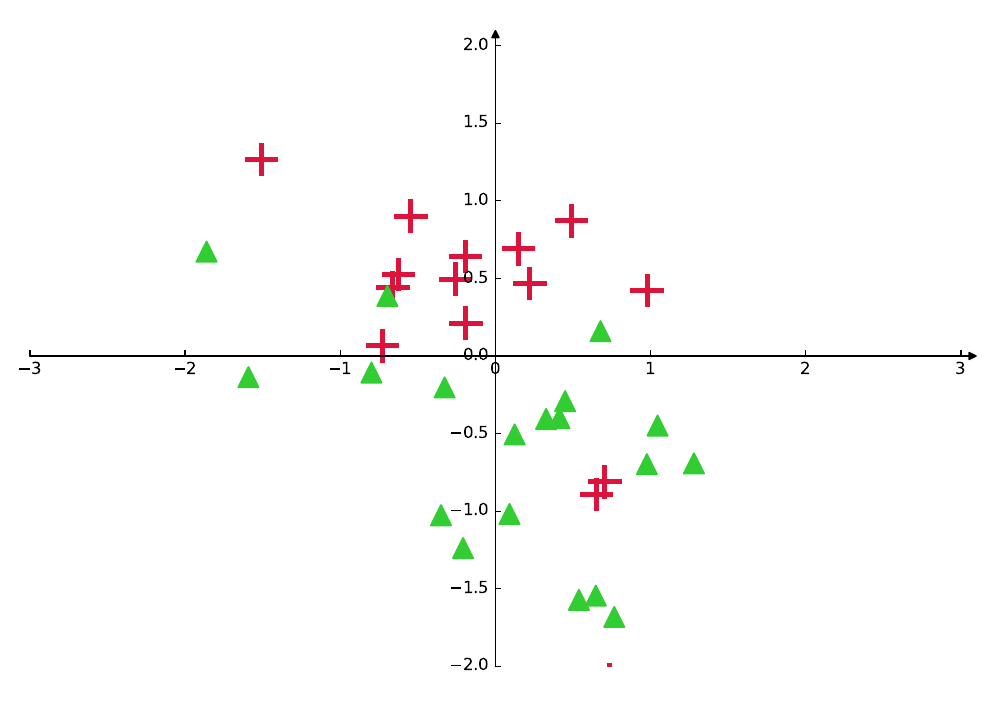
\includegraphics[width=\textwidth]{images/data.png}}
    \only<2>{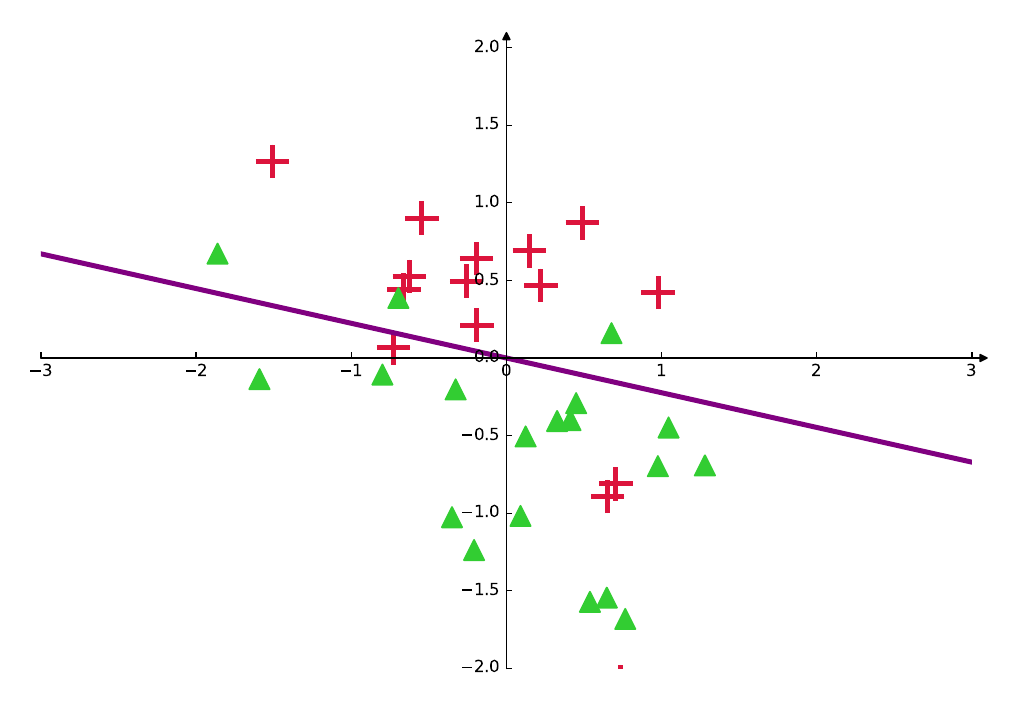
\includegraphics[width=\textwidth]{images/classifpb.png}}
  \end{minipage}%
  ~~~~~~
  \begin{minipage}{0.4\linewidth}
    \only<2>{
      The resulting model:
      \begin{itemize}
      \item is (quite) accurate
      \item contains info on data
      \end{itemize}
    }
  \end{minipage}
\end{frame}


\begin{frame}{Privacy Issues?}
  \begin{minipage}{0.4\linewidth}
    Membership Inference:
    \begin{center}
      \textit{``determine whether a given
      record was part of a model’s
      training dataset''}
    \end{center}
  \end{minipage}%
  ~~~~~~
  \begin{minipage}{0.5\linewidth}
    \only<1>{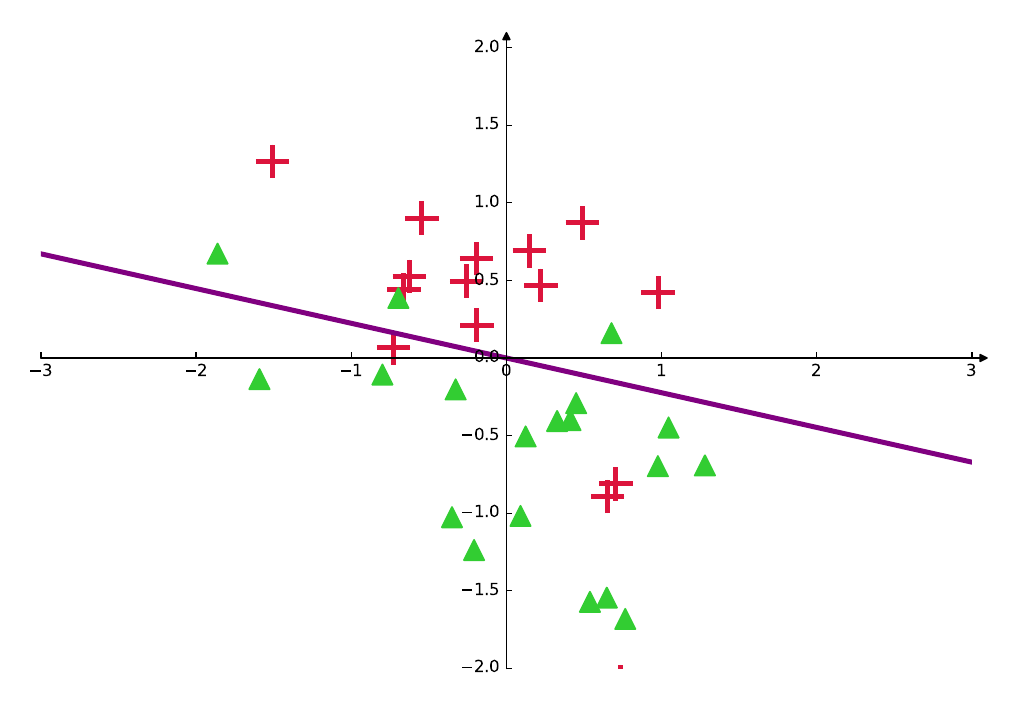
\includegraphics[width=\textwidth]{images/classifpb.png}}
    \only<2>{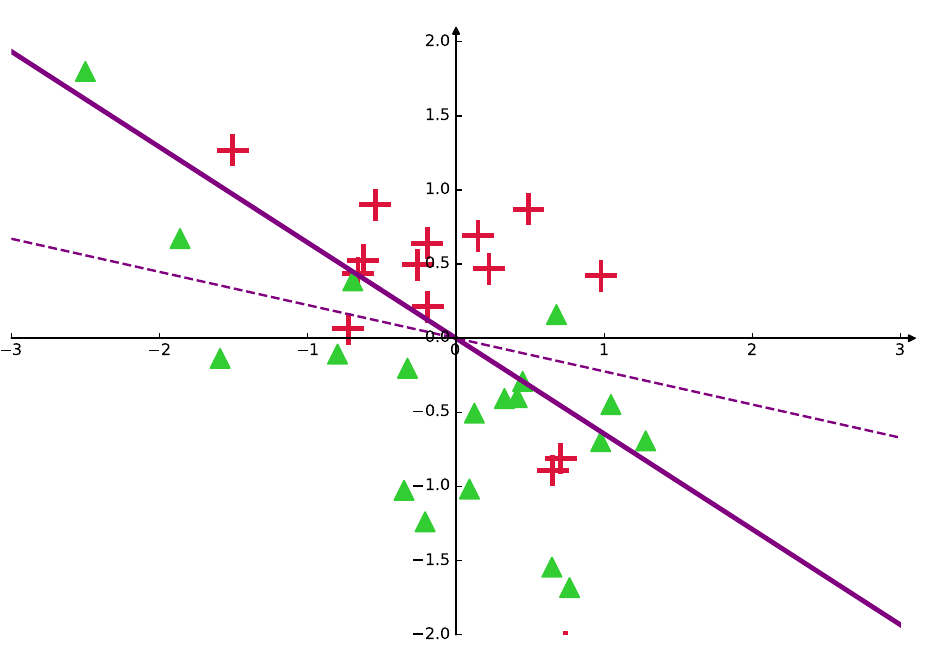
\includegraphics[width=\textwidth]{images/classif-model2.png}}
  \end{minipage}
\end{frame}


\begin{frame}[t]{Guaranteeing Privacy}
  Perturb the predictor with a Gaussian noise $b$:
  \only<1>{
    \begin{align*}
      h_{w}(x) = w_0 + w_1 \cdot x_1 + \cdots + w_p \cdot x_p
    \end{align*}
  }\only<2,3>{
    \begin{align*}
      h_{w+b}(x) = w_0 + \textcolor{purple}{b_0} + (w_1 + \textcolor{purple}{b_1}) \cdot x_1 + \cdots + (w_p + \textcolor{purple}{b_p}) \cdot x_p
    \end{align*}
  }
  \only<3>{
    
\includegraphics[width=2em]{images/check.png}
    noise gives plausible deniability $\rightarrow$ better privacy

    \vspace{-1em}

    
\includegraphics[width=2em]{images/cross.png}
    ~noisy predictions $\rightarrow$ lower accuracy
}
\end{frame}


\begin{frame}{How Strong is the Protection?}
  $\mathcal{A} : D \mapsto w$ is $(\epsilon, \delta)$-differentially private\footfullcite{dwork2006Differential}
  \begin{align*}
    \mathbb{P}(\mathcal{A}(D) \in \mathcal{S})
    \le
    \exp(\epsilon)
    \mathbb{P}(\mathcal{A}(D') \in \mathcal{S})
    + \delta
  \end{align*}
  for all datasets $D, D'$ that differ on one element, and any set $\mathcal{S}$

  \vspace{1em}

  Rule of thumb: $\epsilon \le 1$, $\delta = o(1/|D|)$
\end{frame}

\begin{frame}{How About Fairness?}
  \begin{minipage}{0.5\linewidth}
    \only<1>{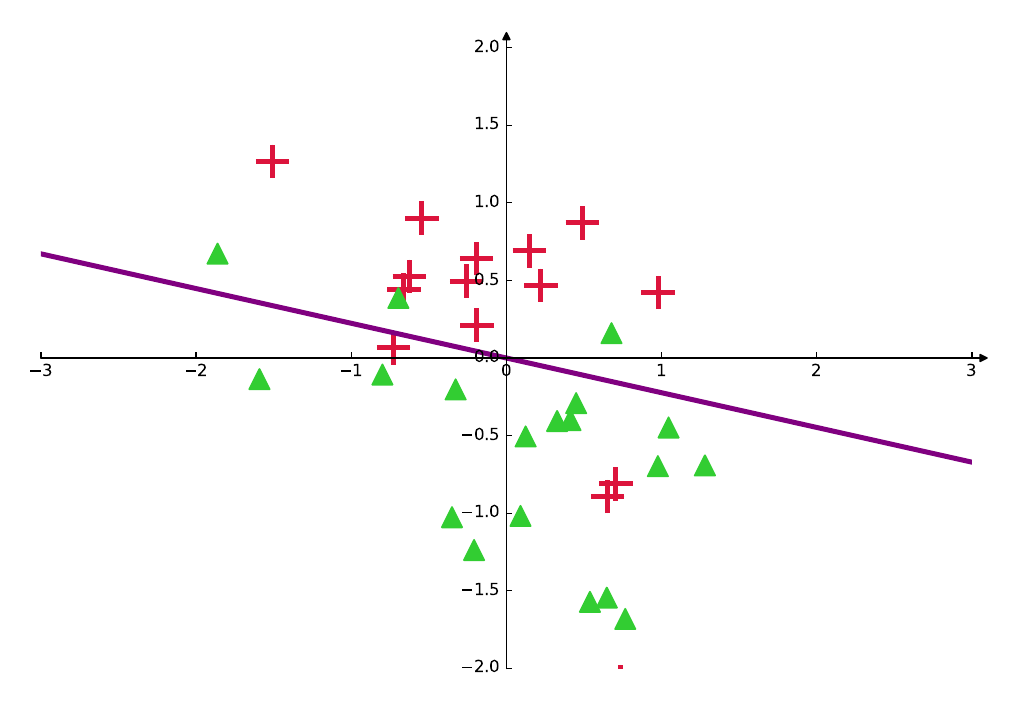
\includegraphics[width=\textwidth]{images/classifpb.png}}
    \only<2,5>{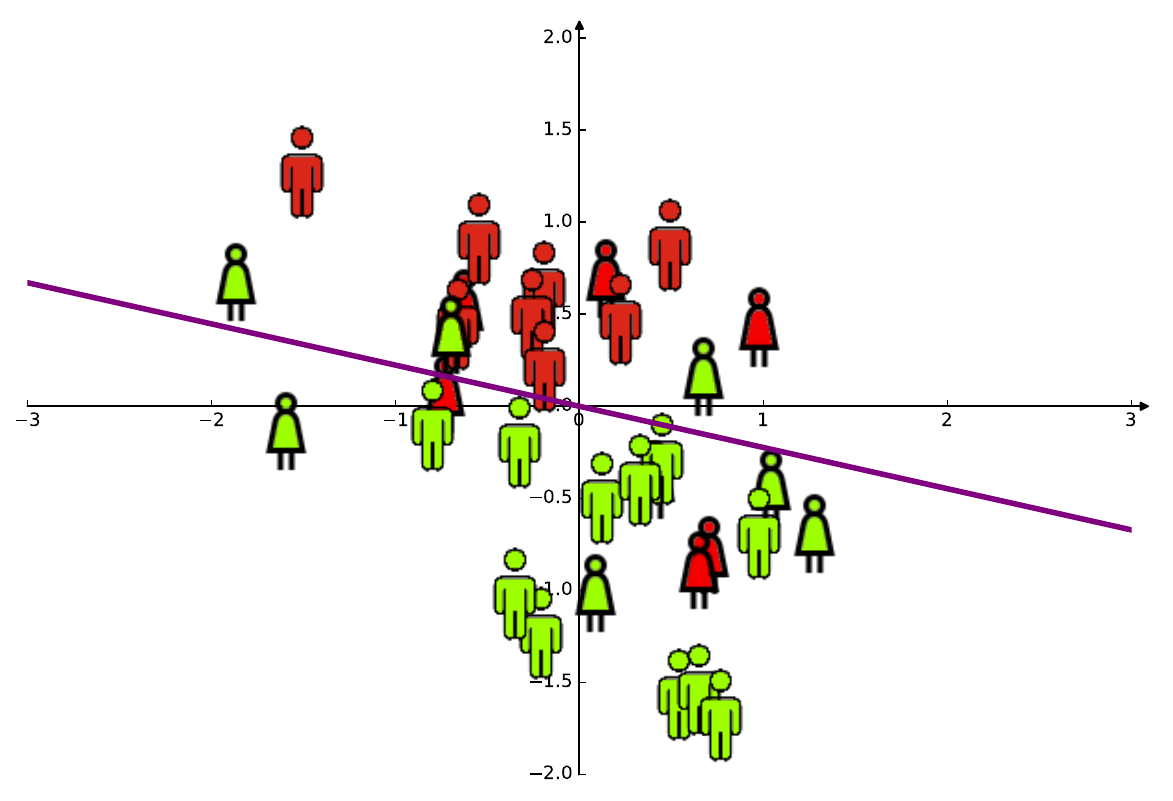
\includegraphics[width=\textwidth]{images/dataset-fairness.png}}
    \only<3>{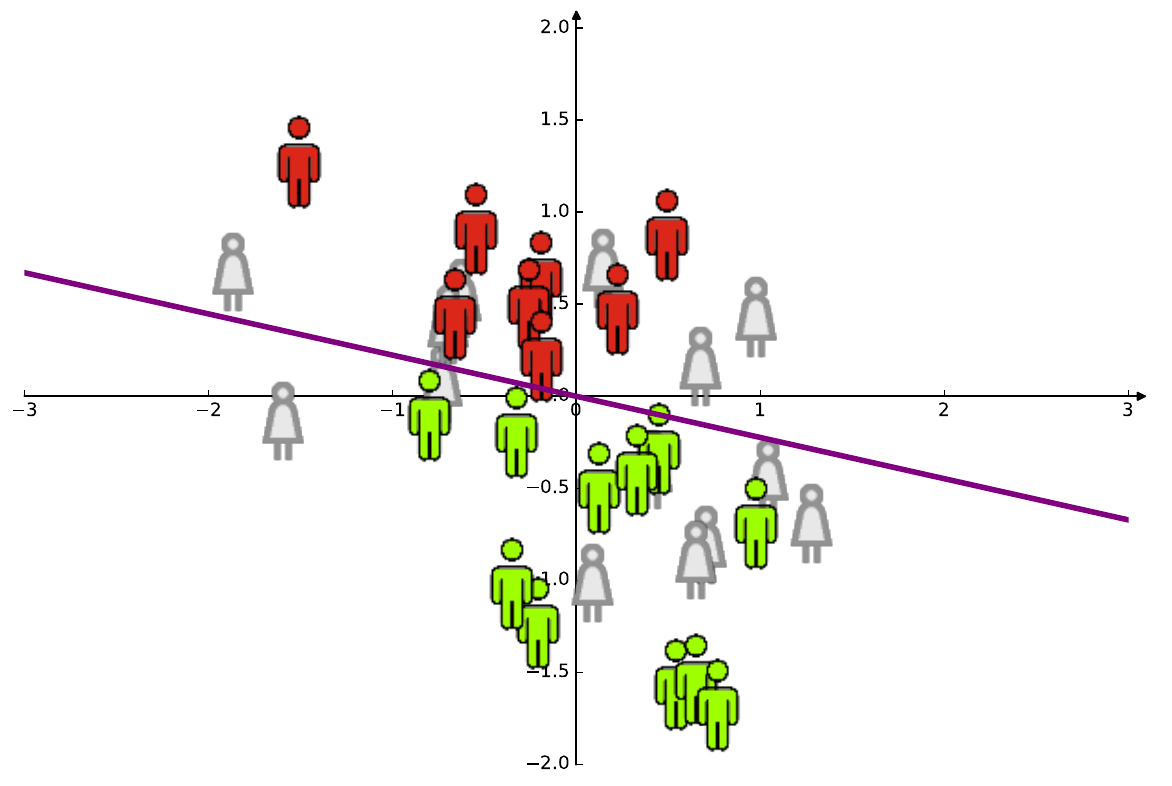
\includegraphics[width=\textwidth]{images/dataset-shirts.png}}
    \only<4>{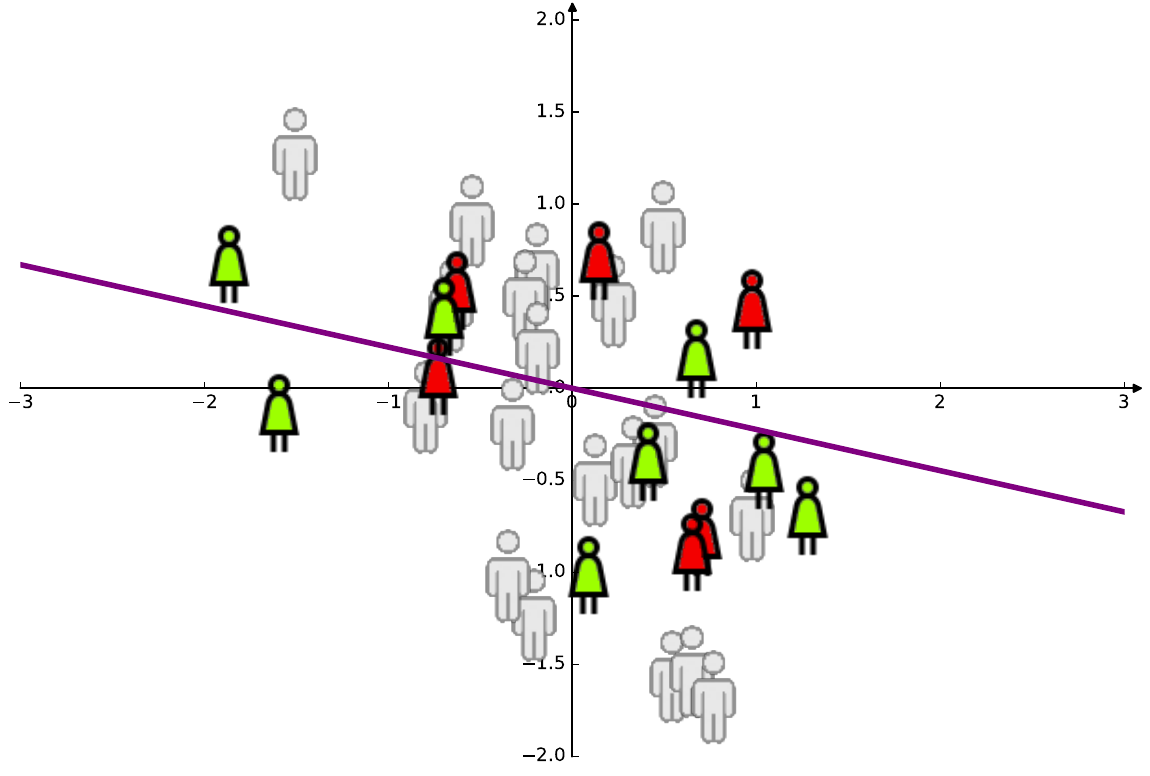
\includegraphics[width=\textwidth]{images/dataset-dress.png}}
  \end{minipage}%
  ~~~~~~
  \begin{minipage}{0.4\linewidth}
    Group Fairness:
    \begin{center}
      \textit{different groups can be treated differently}
    \end{center}
  \end{minipage}%

  \vspace{-2em}

  \only<5>{Note: perturbing the model can have disparate impact\footfullcite{bagdasaryan2019Differential}}

  \vspace{1em}

\end{frame}


\begin{frame}{Modelling the Problem\\[-0.5em]
  \large with a sensitive group $\mathcal{S}$}
  \begin{minipage}{0.5\linewidth}
    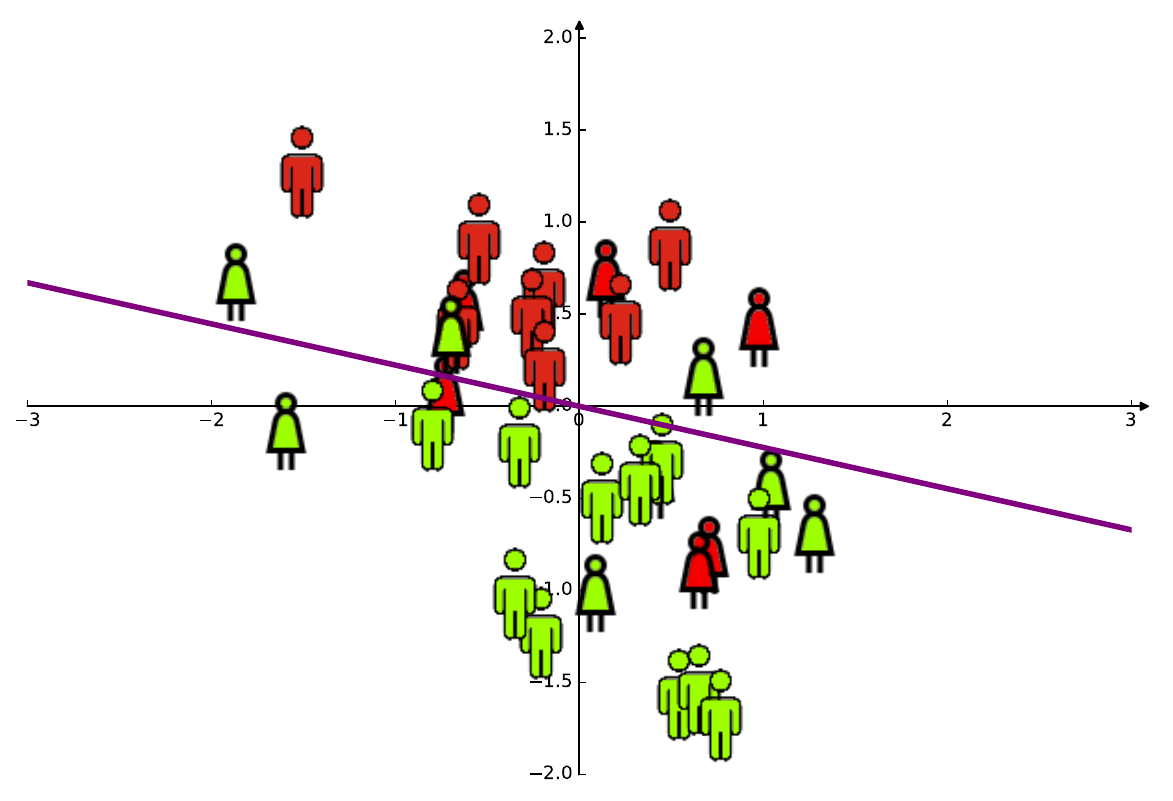
\includegraphics[width=\textwidth]{images/dataset-fairness.png}
  \end{minipage}%
  ~~~~~~
  \begin{minipage}{0.4\linewidth}
    Take: $\mathcal{X} \times \mathcal{S} \rightarrow \{0, 1\}$

    \vspace{1em}

    \textbf{Goal:} learn $h : \mathcal{X} \rightarrow \mathbb{R}$

    \vspace{0.5em}

    $\rightarrow$ classify $x \in \mathcal{X}$ as
    
    \vspace{-1.5em}

    \begin{align*}
      \hat{y} = \sign{h(x)}
    \end{align*}
  \end{minipage}%
\end{frame}


\begin{frame}{Measuring Group Fairness}
  Example: Demographic Parity\footfullcite{calders2009Building}
  \begin{align*}
    F_k(h) =
    \tikz[baseline,remember picture]{\node[fill=red!20,anchor=base]
    (shirtprob){$\displaystyle \prob( h(X) > 0 | S = k)$};}
    -
    \tikz[baseline,remember picture]{\node[fill=red!20,anchor=base]
    (baseprob){$\displaystyle \prob( h(X) > 0 ) $};}    
%    \mathbb{P} (h(X) > 0 | S = k) -  \mathbb{P} (h(X) > 0)
  \end{align*}
  ~~~~~~~~~~~~~~~~~~~~~
  \begin{minipage}{0.3\linewidth}
    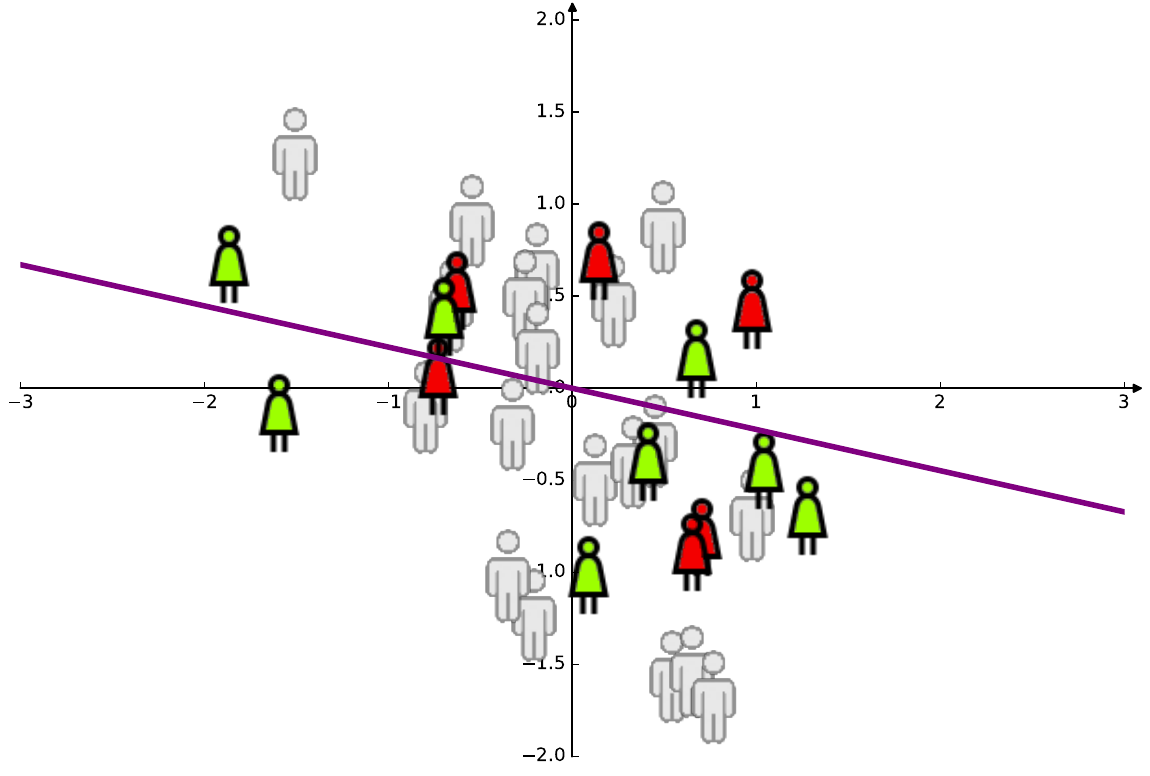
\includegraphics[width=\textwidth]{images/dataset-dress.png}
  \end{minipage}%
  ~~
  \begin{minipage}{0.3\linewidth}
    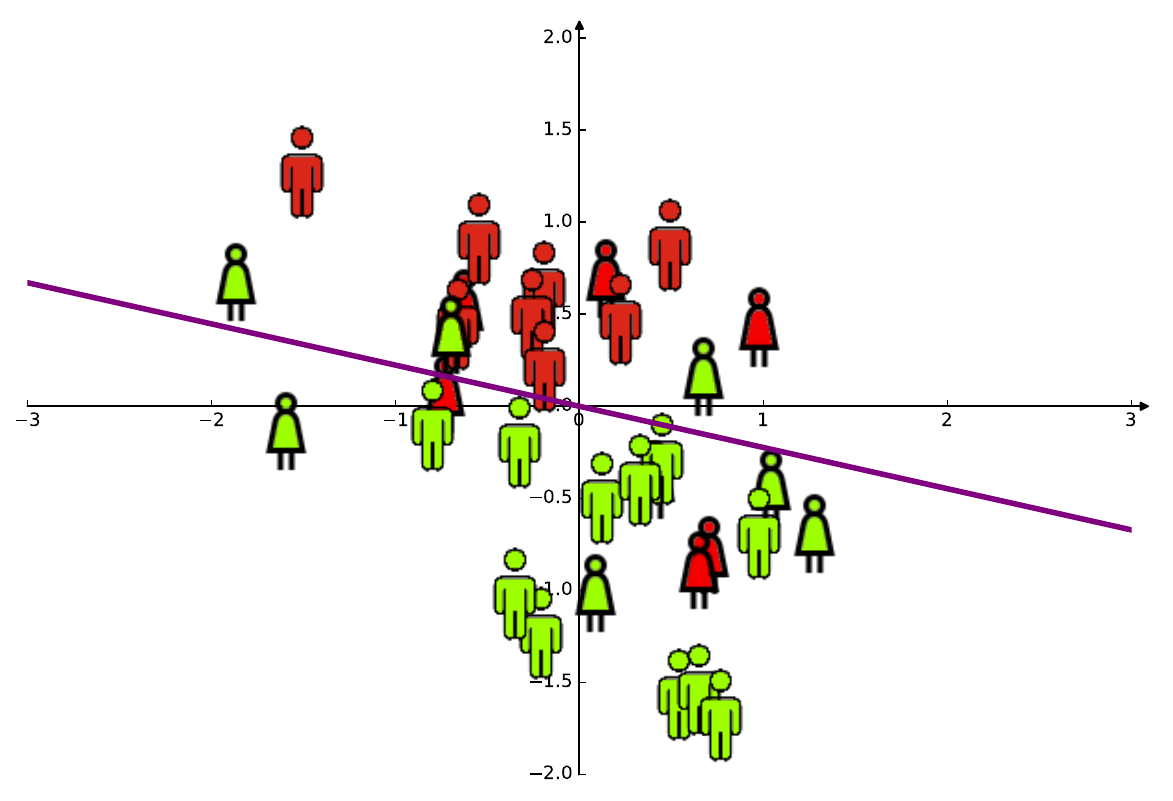
\includegraphics[width=\textwidth]{images/dataset-fairness.png}
  \end{minipage}%

  \vspace{1em}

\end{frame}

\begin{frame}{Fairness and Privacy \\
    \large How much can fairness be affected by privacy?}
  \vspace{-1em}
  \begin{center}
    \only<1>{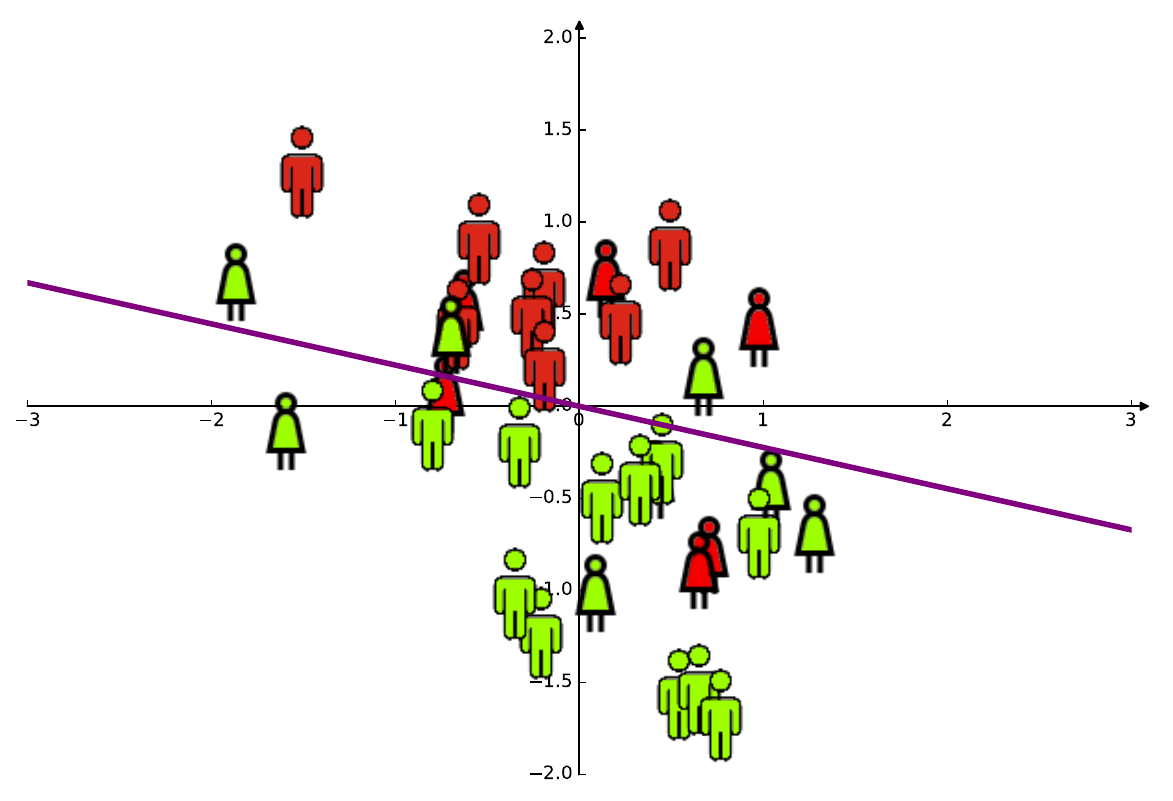
\includegraphics[width=0.6\textwidth]{images/dataset-fairness.png}}%
    \only<2>{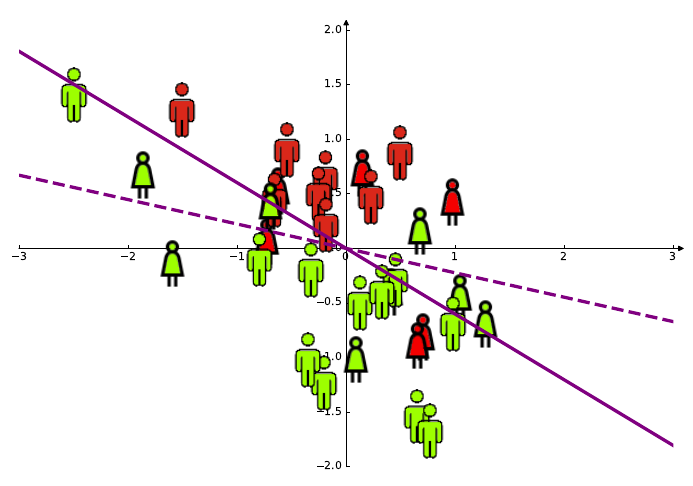
\includegraphics[width=0.6\textwidth]{images/dataset-model2-fairness.png}}%
    \only<3>{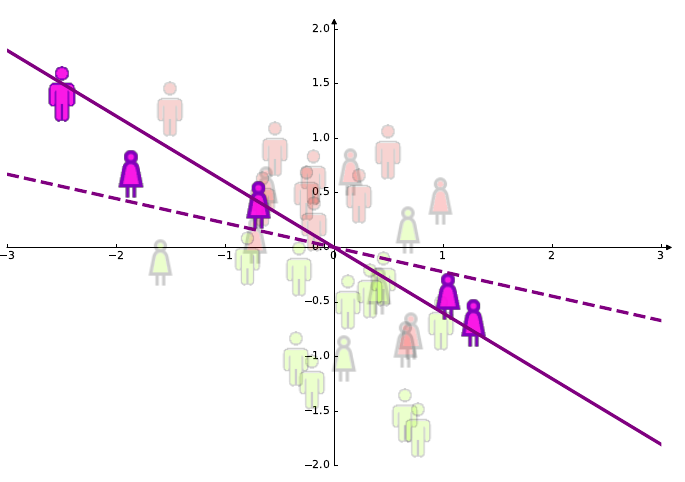
\includegraphics[width=0.6\textwidth]{images/dataset-model2-diff-fairness.png}}%
    
  \end{center}
\end{frame}


\begin{frame}{Fairness and Privacy \\
    \large How much can fairness be affected by privacy?}
  \begin{minipage}{0.5\linewidth}
    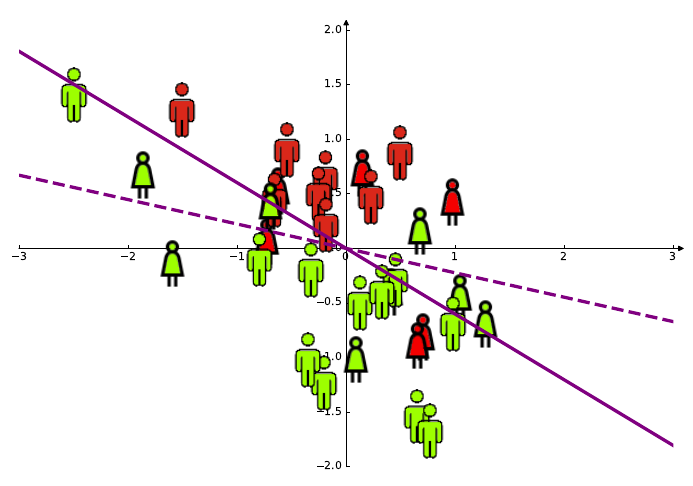
\includegraphics[width=\textwidth]{images/dataset-model2-fairness.png}
  \end{minipage}%
  ~~~~~~
  \begin{minipage}{0.5\linewidth}
    Key assumption:
    \begin{center}
      \textit{confidence margin is lipschitz}
    \end{center}

    \vspace{-1.5em}
    
    \begin{align*}
      | h(x) - h(x') | \le L_{x,y} \norm{ h - h' }
    \end{align*}
    ~~~~~~~~~~~~~for $x, y \in \mathcal{X} \times \{0, 1\}$
  \end{minipage}%
\end{frame}



\begin{frame}{Bound on Difference of Fairness}
  Difference of Fairness
  \begin{align*}
    | F_k(h) - F_k(h') |
    \le
    \chi_k (h) \norm{ h - h' }
  \end{align*}

  Where $\chi_k(h) = \mathbb{E}\Big( \frac{L_{X,Y}}{| h(X) |} ~\Big|~ S = k \Big)
  + \mathbb{E}\Big( \frac{L_{X,Y}}{| h(X) |} \Big)$
\end{frame}


\begin{frame}{Loss of Fairness due to Privacy is Bounded} 
  \vspace{-0.5em}

  Take $h = h_{\text{priv}}$ and $h'= h_\star$:
  \begin{align*}
    | F_k(h^{\text{priv}}) - F_k(h_\star) |
    \le
    O\left(
    \chi_k (h^{\text{priv}}) \frac{\sqrt{p}}{n \epsilon}
    \right)   
  \end{align*}
  Since from DP literature (assuming strongly convex loss)\footfullcite{bassily2014Private}
  \begin{align*}
    \norm{ h_{\text{priv}} - h_\star} \le O\left( \frac{\sqrt{p}}{n \epsilon} \right) \qquad \text{ w.h.p.}
  \end{align*}

  \vspace{-1em}
  
  \Large
  $\Rightarrow$ No need to know optimal model $h_\star$!
  
  \vspace{0.5em}
\end{frame}


\begin{frame}{Numerical Illustration\\[-0.5em]
  \Large Not super tight, but meaningful!}
  \begin{minipage}{0.5\linewidth}
    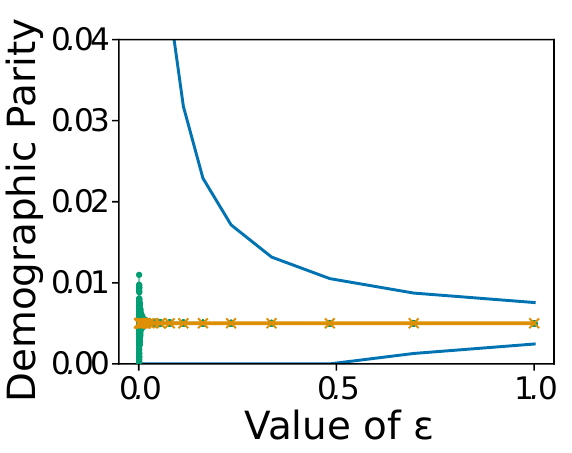
\includegraphics[width=\textwidth]{images/numeric.png}
    
\includegraphics[width=\textwidth]{images/legend.png}
  \end{minipage}%
  ~~~~~~
  \begin{minipage}{0.5\linewidth}
    \begin{itemize}
    \item folktables dataset
    \item $n= 182, 339$ records
    \item $p = 40$ features
    \item Green = real private models
    \end{itemize}
  \end{minipage}%  
\end{frame}


\begin{frame}{Summary}
Fairness of private models:
\begin{itemize}
\item is “close” to the one of non-private model
\item is influenced by confidence margin of the model
\end{itemize}

More results: for other group fairness measures, multi-class problems...

Open questions: use fairness-promoting methods, broader
study of large-margin classifiers...

\end{frame}

\begin{frame}
  \begin{center}
    \vspace{3em}

    \Huge
    Thank you! :)
    
    Questions?

  \end{center}
    \small
    See the Paper:\\[0.5em]

    ~~~~\fullcite{mangold2023Differential}
\end{frame}

\end{document}
%%% Local Variables:
%%% mode: latex
%%% TeX-master: t
%%% End:
